\section{Exempelskript för viktad minsta-kvadrat anpassning}
\label{sec:matlab-wls}
Nedan finner ni två Matlab skript ({\tt wls.m}) för viktad minsta-kvadrat 
(weighted least square) anspassning av en rät linje till en serie punkter med
uppskattad osäkerhet för varje separat punkt.

\subsection{Kod baserad på manuell lösning}

\matlabcode{matlab/wls_manual.m}

\begin{terminaloutput}
>> wls_manual

c_ols =

   2.7426
   3.0403

c_wls =

   2.3613
   3.2790

wrmsd_ols =  1.4769
wrmsd_wls =  0.82180

\end{terminaloutput}


\subsection{Kod baserad på ``fit''}
Ett alternativ till att ställa upp matrisekvationerna för WLS
är att använda 'poly1' i fit:

\matlabcode{matlab/wls.m}

\begin{terminaloutput}
>> wls

k = 3.2790
m =  2.3613
dk = 0.2285
dm = 0.9660
\end{terminaloutput}

Notera att vi även tog fram nya felgränser (en standardavvikelse vilket
motsvarar ett 68.27\% konfidensintervall) på våra två
parametrar. \cref{fig:matlab-wls} visar den genererade plotten.

\begin{figure}
  \centering
  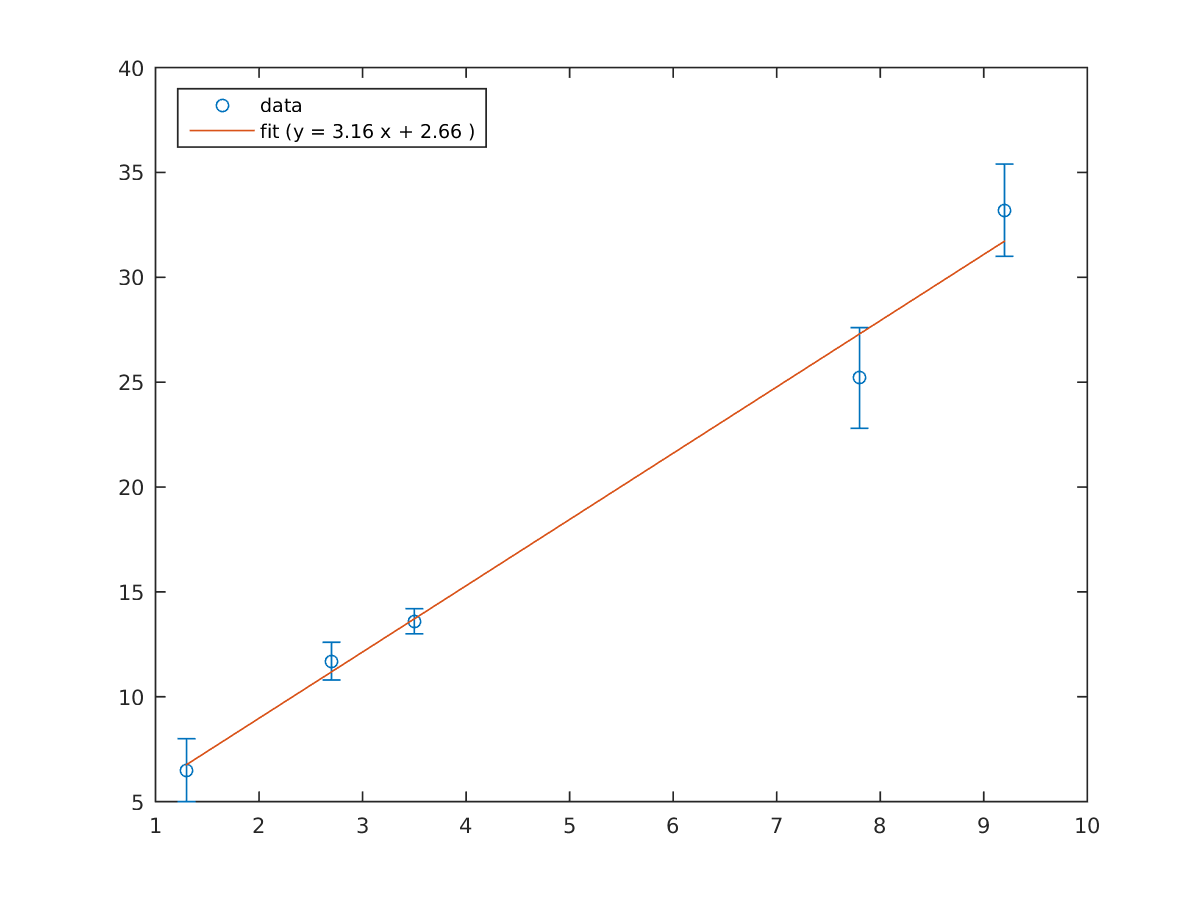
\includegraphics[scale=0.5]{matlab/wls_fit.png}
  \caption{Viktad minsta-kvadrat anpassning}
  \label{fig:matlab-wls}
\end{figure}

%%% Local Variables:
%%% mode: latex
%%% TeX-master: "../main"
%%% ispell-local-dictionary: "swedish"
%%% End:
